\newthought{Algebraic representations} are the topic of this note. Transforming a structure into a corresponding algebraic representation enables easier reasoning and unlocks simpler proofs.

We are going to explore two examples of transformations that I call little algebraic delights. They allow reasoning with ordinary algebraic operations on mathematical objects that are not algebraic at first glance. The first example will use indicator functions\footnote{\bibentry{pollard2002user}} to prove set identities and the second example will use formal languages\footnote{\bibentry{eğecioğlu2021lessons}} to count combinatorial objects.

\subsection{Indicator functions of sets}

When you deal with sets, you usually have to do Boolean algebra. Proving identities of expressions of set operations can become really tedious. Let's say we want to prove that the symmetric difference is associative, so given three sets $A, B, C$ we have

$$
(A \triangle B) \triangle C = A \triangle (B \triangle C)
$$

where the symmetric difference is defined as 

$$
A \triangle B = (A \setminus B) \cup (B \setminus A)
$$

The usual approach of proving is to show that the set on the left hand side $(A \triangle B) \triangle C$ is a subset of the right hand side $A \triangle (B \triangle C)$ and vice versa, by tediously following an $x \in (A \triangle B) \triangle C$ and showing that it is also in $A \triangle (B \triangle C)$ and then the reverse.

Instead of that approach let's try something different. Let ${\mathcal{U} = A \cup B \cup C}$ be the union of all the sets participating in the identity we want to prove (our universe). We define an indicator function ${\mathbb{I}_S: \mathcal{U} \to \{0, 1\}}$ for a subset $S \subseteq \mathcal{U}$ of this universe as:

$$
\mathbb{I}_S(x) =  \begin{cases}
   1 & : x \in S\\
   0 & : x \notin S
\end{cases}
$$ 

We can combine indicator functions with arithmetic operations in a point-wise manner in the field $\mathbb{Z}_2$. It's also clear that sets are in a one-to-one correspondence with their indicator function.

Let's look at the indicator functions of some set operations\footnote{These identities are easy to prove. Just remember, the operations are modulo two and are point-wise, so have to hold for every $x$ in the universe. For example, to prove the last identity $\mathbb{I}_{S \triangle T}(x) = \mathbb{I}_S(x) + \mathbb{I}_T(x)$ we can observe that the symmetric difference shouldn't include the intersection of the two sets, ie when both indicator functions are equal to one. The sum of $1 + 1$ is zero modulo two so that works out, etc... Also remember $-1 = 1$ in $\mathbb{Z}_2$.}:

\begin{align*}
\forall x \in \mathcal{U}:\\  
\mathbb{I}_{S \cup T}(x) &= max(\mathbb{I}_S(x), \mathbb{I}_T(x)) \\
\mathbb{I}_{S \cap T}(x) &= \mathbb{I}_S(x) \cdot \mathbb{I}_T(x) \\
\mathbb{I}_{S^c}(x) &= 1 - \mathbb{I}_S(x) \\
\mathbb{I}_{S \setminus T}(x) &= \mathbb{I}_S(x) \cdot (1 - \mathbb{I}_T(x)) \\
\mathbb{I}_{S \triangle T}(x) &= \mathbb{I}_S(x) + \mathbb{I}_T(x) = \mathbb{I}_S(x) - \mathbb{I}_T(x)
\end{align*}

Let's omit the $x$ in these point-wise expressions:

\begin{align*}
\mathbb{I}_{S \cup T} &= max(\mathbb{I}_S, \mathbb{I}_T) \\
\mathbb{I}_{S \cap T} &= \mathbb{I}_S \cdot \mathbb{I}_T \\
\mathbb{I}_{S^c} &= 1 - \mathbb{I}_S \\
\mathbb{I}_{S \setminus T} &= \mathbb{I}_S \cdot (1 - \mathbb{I}_T) \\
\mathbb{I}_{S \triangle T} &= \mathbb{I}_S + \mathbb{I}_T = \mathbb{I}_S - \mathbb{I}_T
\end{align*}

Since we agreed that we will work with the indicator functions of the sets, we could just drop the $\mathbb{I}$ from the notation\footnote{To parse expressions where we dropped the symbol $\mathbb{I}$, we have to group set operations and imagine an $\mathbb{I}$ in front of them, ie set operations have grouping precedent over arithmetic operations. For example $S \cup T \cdot V$ means the point-wise multiplication $\mathbb{I}_{S \cup T} \cdot \mathbb{I}_V$.}:

\begin{align*}
S \cup T &= max(S, T) \\
S \cap T &= S \cdot T \\
S^c &= 1 - S \\
S \setminus T &= S \cdot (1 - T) \\
S \triangle T &= S + T = S - T
\end{align*}

Given the indicator function equivalent of the symmetric difference, our initial $(A \triangle B) \triangle C = A \triangle (B \triangle C)$ becomes the almost trivial ${(A + B) + C = A + (B + C)}$.

The expression for the union has $max$ which is sometimes convenient but sometimes gets in the way of point-wise arithmetic. But we can get rid of it by observing that the union is the symmetric difference plus the intersection:

$$
S \cup T = S \triangle T + S \cdot T = S + T + S \cdot T
$$
 
Let's deploy our new-found powers to something more complicated and try to prove that

$$
(\bigcap_{i = 1}^n A_i) \triangle (\bigcap_{i = 1}^n B_i) \subseteq \bigcup_{i = 1}^n (A_i \triangle B_i)
$$

Two things before we start: our universe expanded to ${\mathcal{U} = (\bigcup_{i = 1}^n A_i) \cup (\bigcup_{i = 1}^n B_i)}$ and we have for subsets $S, T \subseteq \mathcal{U}$:

$$
S \subseteq T \Leftrightarrow \forall x \in \mathcal{U}: \mathbb{I}_S(x) \leq \mathbb{I}_T(x)
$$

Given that inequality and the fact that the range of indicator functions is $\{0,1\}$, when the right-hand side is one then the inequality is trivially true. The only interesting case is when the right-hand side is zero. We use the $max$ expression for union and have 

$$
\bigcup_{i = 1}^n (A_i \triangle B_i) = max_{i = 1}^n (A_i - B_i)
$$

This max can only be zero iff all $A_i = B_i$. But in that case we also have the left-hand side zero because the left-hand side is

$$
(\bigcap_{i = 1}^n A_i) \triangle (\bigcap_{i = 1}^n B_i) = \prod_{i = 1}^n A_i - \prod_{i = 1}^n B_i
$$

which concludes our proof.

\subsection{Formal Languages to count combinatorial objects}

We will do a very quick, (ahem) informal introduction to Formal Languages\footnote{This should be very familiar for all of us computer science majors.}. We start with an alphabet $\mathcal{A}$ which is an ordered set of symbols. We want it ordered so that we can do lexicographic ordering of words from that alphabet. Speaking of words: they are sequences of symbols from the alphabet. Concatenation of two words $w_1$ and $w_2$ is denoted by $w_1 \cdot w_2$ and defined as you would expect. The empty word $\epsilon$ has length zero and is the neutral element of concatenation. A word $w_2$ is a prefix of a word $w_1$ iff there is a word $w_3$ such that $w_1 = w_2 \cdot w_3$. The set of all words (including the empty word $\epsilon$) from alphabet $\mathcal{A}$ is denoted $\mathcal{A}^*$ and the set of all words excluding $\epsilon$ is $\mathcal{A}^+$. A subset $\mathcal{L} \subseteq \mathcal{A}^*$ is called a language.

We have a couple of ways to form new languages from given ones. One way is concatenation. Given $\mathcal{L}_1, \mathcal{L}_2$:

$$
\mathcal{L}_1 \cdot \mathcal{L}_2 = \{w_1 \cdot w_2: w_1 \in \mathcal{L}_1, w_2 \in \mathcal{L}_2\}
$$

The other way is the set union $\mathcal{L}_1 \cup \mathcal{L}_2$ which becomes more interesting when $\mathcal{L}_1$ and $\mathcal{L}_2$ are disjoint.

So far so good. Now comes the cool stuff. Given a language $\mathcal{L}$ we define its listing series as:

$$
s\mathcal{L} = \sum_{w \in \mathcal{L}} w
$$

Some notes on this notation: This is a formal sum and should not be thought of as the normal addition of numbers. The name \emph{listing series} hints at its special nature: it lists out the words of a language in a chain. Using the plus symbol as the chain separator (as opposed to say the comma) might be confusing in the beginning but it will pay off later when it is combined with the multiplication symbol used for concatenation. The words in the sum are usually listed out in lexicographic order. The usefulness of the listing series will become apparent when we relate it to concatenation. Let's look at an example: $\mathcal{L}_1 = \{a, b\}$:

$$
s\mathcal{L} = aa + ab + ba + bb
$$

We take a second language $\mathcal{L}_2 = \{c\}$ and now list out the concatenation (the listing operator \emph{s} has lower precedent than the concatenation operator, saving us round braces):

\begin{align*}
s \mathcal{L}_1 \cdot \mathcal{L}_2 &= aac + abc + bac + bbc \\
                                    &= (aa + ab + ba + bb) \cdot c \\
                                    &= (s \mathcal{L}_1) \cdot (s \mathcal{L}_2)
\end{align*}

Treating $+$ and $\cdot$ in a strictly symbolic, algebraic way, it looks like $\cdot$ distributes over $+$ and preserves the correct meaning of listing series of the languages involved in the expression. Note that unlike with the multiplication of numbers, concatenation is not commutative, so $ab$ and $ba$ are different and $aa + ab + ba + bb$ is not $aa + 2ab + bb$ (that $2$ in the last expression doesn't even make sense). We have to be careful not to cross the line and conflate the operations with the familiar numeric ones, but if we are careful we can now manipulate languages algebraically as if they were finite sums of terms (or even infinite sums as we will see).

Before we can put this to good use, let us also introduce another notational convenience: exponentiation. We have seen that $ab$ and $ba$ are not the same, also $aab$ and $baa$ are different. But as a convenience we can abbreviate $aa$ to $a^2$ and in general a word $aa\ldots a$ of length $n$ formed with one single symbol $a$ as $a^n$. That way $aab$ and $baa$ can be written $a^2b$ and $ba^2$ respectively.

Exponentiation can be expanded to languages: $\mathcal{L}^n$ is the language formed by concatenating $\mathcal{L}$ with itself $n$ times. We also agree that
$\mathcal{L}^0 = \{\epsilon\}$.
 
One last thing before we start: what should the placeholder symbol for the empty word in a listing series be? Well, since the empty word is the neutral element of concatenation and we use "multiplication" as our concatenation operator, it is befitting to use $1$ for the empty word and this also fits with distribution of concatenation over listing series and our "exponentiation". For a neat example: consider $\mathcal{A} = \{a\}$ and list out $\mathcal{A}^*$(purely symbolic\footnote{With a wink towards calculus, we agree that $\frac{1}{1 - a}$ symbolizes the listing series of $\mathcal{A}^*$.}):

$$
s \mathcal{A}^* = 1 + a + a^2 + a^3 + \ldots = \sum_{i = 0}^\infty a^i = \frac{1}{1 - a}
$$

We're ready to do some interesting combinatorics. Until now we used the subscript on a language symbol like $\mathcal{L}_1$ just to make it an individual and distinguish it from another language $\mathcal{L}_2$ in this exposition. From now on we will give it meaning: given a fixed alphabet we say $\mathcal{L}_n$ is the language of all the words with length $n$ from that alphabet.

It's not that hard to prove that when $n = p + q$ with $n, p, q \in \mathbb{N}$ then (over the same alphabet):

\begin{align*}
\mathcal{L}_n &=  \mathcal{L}_p \cdot \mathcal{L}_q \\
s \mathcal{L}_n &= (s \mathcal{L}_p) \cdot (s \mathcal{L}_q)
\end{align*}

This is really powerful because it is a rich source of recursions for both the listing series generation and for counting the number of words in the language.

Consider the alphabet of two symbols: $\mathcal{A} = \{a, b\}$. Let's list out some languages of different lengths from this alphabet:

\begin{align*}
s \mathcal{L}_0 &= 1 \\
s \mathcal{L}_1 &= a + b \\
s \mathcal{L}_2 &= aa + ab + ba + bb \\
s \mathcal{L}_3 &= aaa + aab + aba + baa + abb + bab + bba + bbb \\
\ldots
\end{align*}

We observe that $s \mathcal{L}_n = s (a \cdot \mathcal{L}_{n-1}) + s (b \cdot \mathcal{L}_{n-1})$ and if $\mathcal{L}_{n-1}$ is listed in lexicographic order, then this recursion even preserves the lexicographic order. In essence, it gives us an algorithm to generate words of a given length in lexicographic order\footnote{It also lets us count the number of words in $\mathcal{L}_n$: if $b_n = |\mathcal{L}_n|$ is the number of words in $\mathcal{L}_n$, then it satisfies the recursion: $b_n = 2 b_{n-1}$ and we know $b_0 = 1$. So no surprise here: $b_n = 2^n$.}.

Let us expand the language subscript notation with even more meaning. Same two-symbol alphabet $\mathcal{A} = \{a, b\}$, and now $\mathcal{L}_{n,k}$ means language of words of length $n$ with exactly $k$ $b$'s in them. Then\footnote{If a word of length $n$ with exactly $k$ $b$'s starts with an $a$ then it must be followed by a word of length $n-1$ with $k$ $b$'s. If on the other hand it starts with a $b$ then it must be followed by a word of length $n-1$ with $k-1$ $b$'s.}:

$$
s \mathcal{L}_{n, k} = (s \ a \cdot \mathcal{L}_{n-1, k}) \cdot (s \ b \cdot \mathcal{L}_{n-1, k-1})
$$

If we denote the size of language $\mathcal{L}_{n, k}$ with $C_{n, k} = |\mathcal{L}_{n, k}|$ then we have the recursion:

$$
C_{n, k} = C_{n-1, k} + C_{n-1, k-1}
$$

and the astute reader recognizes this as the recursion of the binomial coefficients and the Pascal triangle.

If we find a one-to-one correspondence between the combinatorial objects that we want to reason about and words in a language, then we can deploy this formal language machinery to generate the objects (using listing series) and also count them.

As an example of such a correspondence, consider a $n \times m$ lattice grid and East/North lattice paths on that grid.

\begin{figure}[t]
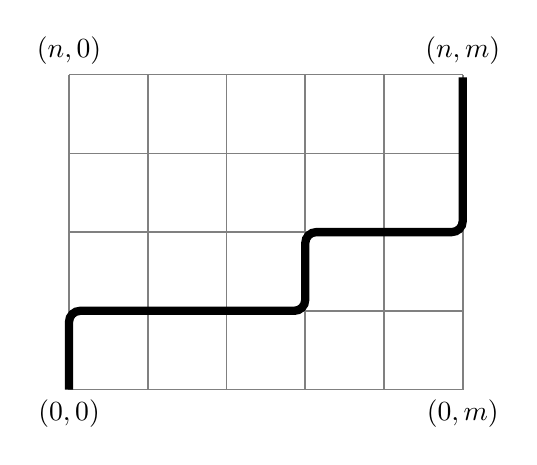
\begin{tikzpicture}[
      shorten > = 1pt, % don't touch arrow head to node
      auto,
      node distance = 3cm, % distance between nodes
      semithick % line style
  ]
  
 \draw[step=1cm, color=gray] (0, 0) grid (5, 4);

\foreach \coord/\label [count=\xi] in {
    {0,0}/{$(0, 0)$},
    {5,4}/{$(n, m)$},
    {5,0}/{$(0, m)$},
    {0,4}/{$(n, 0)$}
}{
    \pgfmathsetmacro\anch{mod(\xi,2) ? "north" : "south"}
    \node[anchor=\anch] at (\coord) {\label};
}

\draw[line width=3pt, rounded corners] (0,0) -- (0,1) -- (3,1) -- (3,2) -- (5,2) -- (5,4);

\end{tikzpicture}
\caption{Lower left corner of grid is $(0, 0)$ and upper right corner is $(n, m)$. Paths are going either up North or right East, always along an edge in the grid.}
\end{figure}

How many such paths are there that go from $(0, 0)$ to $(n, m)$ ? We can make a one-to-one correspondence from the set of possible paths to a language with the two-symbol alphabet $\{E, N\}$ ($E$ for East, $N$ for North). Each path has to have $n + m$ segments with $n$ North-going segments and $m$ East-going segments. The corresponding language $\mathcal{L}$ over the alphabet $\mathcal{A}= \{E, N\}$ consists of words of length $n + m$ with exactly $n$ $N$'s (and therefore $m$ $E$'s). We recognize again the binomial coefficient and have the number of paths

$$
|\mathcal{L}| = C_{n + m, n}
$$

 This was a simple example but the general idea stays the same: find a bijection between the combinatorial objects and words in a language over some alphabet and then switch to algebraic series manipulation of the words. For example, if it is a 3-dimensional lattice grid, then we expand the alphabet to three symbols and proceed. Sometimes the language used in the correspondence has very interesting restrictions such as in a two-symbol alphabet language where the number of $a$'s and $b$'s has to be equal and any prefix of the word has to have at least as many $a$'s as $b$'s\footnote{Words from such a language are called Dyck words. These words have correspondence to many combinatorial objects.}. 

